\chapter{Návrh a realizace, zhodnocení výsledků}
\label{sec:realizace}

Tato kapitola detailně popisuje praktickou část bakalářské práce. Text je strukturován přesně podle fází vývoje prototypu: od fyzického návrhu hardwaru, přes implementaci softwarových nástrojů pro generování a analýzu provozu, až po finální zhodnocení dosažených výsledků v laboratorním prostředí.

\section{Návrh přenosného zařízení}
\label{sec:navrh_zarizeni}

Pro zajištění dostatečného výpočetního výkonu a kompatibility se síťovými nástroji byl jako hlavní výpočetní jednotka zvolen jednodeskový počítač Raspberry Pi 3 Model B+. Deska je osazena čtyřjádrovým procesorem Cortex-A53 taktovaným na 1,4 GHz, disponuje operační pamětí o velikosti 1 GB, čtveřicí portů USB 2.0 a bezdrátovým rozhraním pracujícím v pásmech 2,4 GHz i 5 GHz \cite{rpi3bplus}. Tato platforma poskytuje nativní podporu pro operační systémy na bázi Linuxu, což je kritický požadavek pro pokročilou manipulaci se síťovými rozhraními a směrováním, a její pořizovací cena odpovídá záměru vytvořit dostupnou alternativu ke komerčním testerům.

Volba platformy s sebou nese jedno omezení, které je nutné znát předem, neboť přímo ohraničuje vypovídací hodnotu měření propustnosti. Integrované ethernetové rozhraní je sice označováno jako gigabitové, je však k procesoru připojeno prostřednictvím sběrnice USB 2.0, a jeho výrobcem udávaná nejvyšší dosažitelná propustnost proto činí 300 Mbps \cite{rpi3bplus}. Totéž omezení platí i pro externí adaptéry popsané dále, které tutéž sběrnici navíc sdílejí. Zařízení tedy nemůže sloužit k ověření, zda linka skutečně přenese plnou gigabitovou rychlost; jeho úlohou je prokázat funkčnost spoje, změřit dosažitelnou propustnost v rámci možností platformy a poskytnout srovnání mezi protokoly za shodných podmínek.

Aby zařízení splňovalo požadavek na přenositelnost a autonomii, je Raspberry Pi osazeno 5palcovým dotykovým displejem (HDMI LCD V2). Napájení displeje a přenos dat z dotykové vrstvy jsou realizovány prostřednictvím GPIO pinů, zatímco obrazový signál je přenášen standardním rozhraním HDMI. Díky tomuto řešení nevyžaduje analyzátor pro svůj provoz připojení externího monitoru, klávesnice ani myši.

Jelikož integrované síťové rozhraní Raspberry Pi nedostačuje pro současné a vzájemně oddělené generování a naslouchání provozu, byla hardwarová architektura rozšířena o dva externí USB/LAN ethernetové adaptéry. Tyto adaptéry se v systému hlásí jako dvě nezávislá rozhraní označená jako \texttt{eth1} a \texttt{eth2}.

První z nich slouží výhradně jako monitorovací rozhraní pro pasivní odposlech sítě. Druhý adaptér je dedikován pro aktivní testování sítě. Fyzické oddělení těchto rolí zabraňuje situaci, kdy by generovaný zátěžový provoz zpětně ovlivňoval statistiky zachycené naslouchajícím rozhraním.

\section{Realizace generátoru a analyzátoru provozu}
\label{sec:realizace_generatoru}

Základním stavebním kamenem softwarové architektury je operační systém založený na jádře Linux. Jelikož analyzátor využívá dvě fyzická síťová rozhraní zapojená do stejného síťového segmentu, vyvstává problém s výchozím směrováním. Tento problém byl úspěšně vyřešen implementací technologie Linux Network Namespaces (netns). V rámci inicializačního skriptu jsou automaticky vytvořeny dva nezávislé jmenné prostory, do kterých jsou přesunuta fyzická rozhraní. Každý prostor disponuje vlastní směrovací tabulkou.

Do obou jmenných prostorů byl dále integrován server dnsmasq. Každá jeho instance obsluhuje výhradně rozhraní vlastního prostoru a přiděluje cílové stanici adresu z odpovídajícího rozsahu, tedy \texttt{10.0.1.20} na straně monitorovacího portu a \texttt{10.0.2.20} na straně portu určeného ke generování provozu. Obsluha protokolu IPv6 je řešena souběžně, prostřednictvím zpráv Router Advertisement s unikátními lokálními prefixy \texttt{fd00:1::/64} a \texttt{fd00:2::/64}. Cílová stanice tak nevyžaduje žádnou předchozí ruční přípravu a k analyzátoru se připojí pouhým zasunutím kabelu. Způsob, jakým stanice adresu získá, se však u obou protokolů zásadně liší; této otázce je věnována podkapitola \ref{sec:autokonfigurace}.

Uživatelské rozhraní je naprogramováno v jazyce Python s využitím knihovny Tkinter. Aplikace plní roli centrálního řídicího panelu (viz Obrázek \ref{fig:gui}) a je rozvržena pro rozlišení displeje 800 na 480 obrazových bodů. Za účelem maximalizace uživatelského komfortu při ovládání přes dotykový displej byla do aplikace naprogramována vlastní virtuální číselná klávesnice (Numpad). Tím zcela odpadá nutnost připojovat k analyzátoru externí hardwarovou klávesnici při zadávání IP adres.

\begin{figure}[htbp]
    \centering
    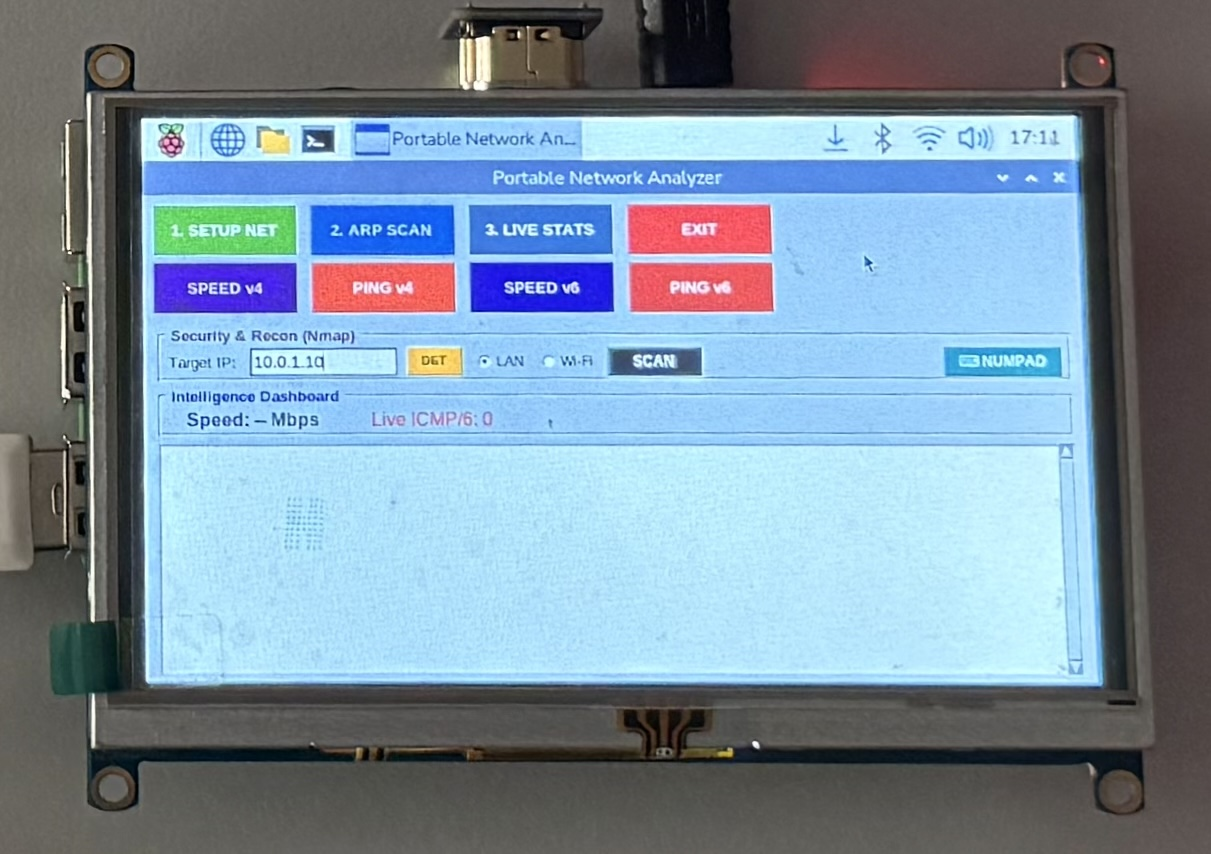
\includegraphics[width=0.8\textwidth]{Figures/gui.JPG}
    \caption{Hlavní obrazovka aplikace Portable Network Analyzer}
    \label{fig:gui}
\end{figure}

Inicializace celého síťového prostředí je spouštěna přímo z aplikace jediným tlačítkem, které vyvolá skript uvedený v Příloze \ref{sec:Appendix1}. Průběh inicializace je uživateli vypisován do textového pole, takže lze bezprostředně ověřit, že oba jmenné prostory vznikly, rozhraní do nich byla přesunuta a obě instance serveru dnsmasq běží (viz Obrázek \ref{fig:setup_net}).

\begin{figure}[htbp]
    \centering
    \includegraphics[width=0.8\textwidth]{Figures/gui_setup_net.JPG}
    \caption{Výstup inicializačního skriptu při vytváření jmenných prostorů}
    \label{fig:setup_net}
\end{figure}

Klíčovým rozšířením softwarové části je integrace bezpečnostního skeneru Nmap pro aktivní síťový průzkum (Network Reconnaissance). Uživatelské rozhraní umožňuje spouštět audity ve dvou režimech: kabelové skenování (LAN) zevnitř izolovaného prostoru a bezdrátové skenování přes integrovaný Wi-Fi modul s funkcí automatické detekce IP adresy výchozí brány.

Pro pasivní odposlech je využíván nástroj tcpdump, pro mapování topologie knihovna Scapy a aktivní zátěžové testy jsou realizovány nástrojem iperf3, odděleně pro protokoly IPv4 a IPv6.

Pasivní monitorování je v aplikaci řešeno tak, aby výsledek byl použitelný okamžitě a bez následného rozboru zachyceného souboru. Odposlech běží v samostatném vlákně, takže uživatelské rozhraní zůstává po celou dobu ovladatelné, a zachycené pakety jsou průběžně tříděny podle protokolu. Obsluha tak na displeji sleduje narůstající počty rámců protokolů TCP, UDP a ICMP a zvlášť vyznačenou přítomnost provozu protokolu IPv6. Toto rozdělení bylo zvoleno záměrně: pro rychlou diagnostiku v terénu je podstatnější okamžitá odpověď na otázku, zda v segmentu vůbec něco komunikuje a jakého druhu provoz převažuje, než úplný výpis obsahu jednotlivých paketů. Zachycený provoz lze zároveň uložit do souboru ve formátu pcap a podrobit jej později rozboru v plnohodnotném analyzátoru na stolním počítači.

Vlastní řešení si vyžádal výběr jmenného prostoru pro spouštěné nástroje. Protože každý testovací port obsluhuje jinou podsíť a mezi oběma prostory neexistuje cesta, nelze nástroj spustit v pevně zvoleném prostoru. Aplikace proto obsahuje metodu \texttt{netns\_for()}, která z adresy zadaného cíle určí, do které podsítě náleží, a příslušný nástroj spustí v odpovídajícím jmenném prostoru. Tento mechanismus je společný pro skener Nmap, testy dostupnosti i zátěžové testy, takže obsluha zadává pouze cílovou adresu a o směrování požadavku se nestará.

\subsection{Adresní autokonfigurace protokolu IPv6}
\label{sec:autokonfigurace}

Požadavek na plnou podporu protokolu IPv6 se při realizaci ukázal jako nejnáročnější část celé konfigurace, a to nikoli kvůli objemu práce, nýbrž kvůli odlišné povaze obou protokolů. Zatímco stanice s protokolem IPv4 nemá bez běžícího klienta DHCP jak adresu získat, protokol IPv6 nabízí vedle stavového serveru DHCPv6 také bezstavovou autokonfiguraci, při níž si stanice sestaví adresu sama z prefixu inzerovaného směrovačem ve zprávě Router Advertisement. Kterou z obou cest stanice zvolí, určuje samotná zpráva: příznak M (Managed address configuration) ji odkazuje na server DHCPv6, zatímco příznak A (Autonomous address configuration), nesený u každého inzerovaného prefixu zvlášť, teprve povoluje sestavení adresy z tohoto prefixu \cite{nastase2024}.

V první realizaci byl rozsah adres zapsán jako jediná konkrétní adresa, tedy \texttt{-{}-dhcp-range=\allowbreak fd00:1::20,\allowbreak fd00:1::20,\allowbreak 64,\allowbreak 12h}. Toto zdánlivě neškodné zúžení rozsahu vedlo k tomu, že server dnsmasq nastavil příznaky ve zprávě Router Advertisement způsobem uvedeným v Tabulce \ref{tab:ra_flags}. Hodnoty byly odečteny přímo na cílové stanici nástrojem \texttt{rdisc6}, který zprávu vyžádá zasláním Router Solicitation a vypíše její obsah v čitelné podobě.

\begin{table}[htbp]
    \caption{Příznaky ve zprávě Router Advertisement před úpravou a po ní}
    \label{tab:ra_flags}
    \centering
    \begin{tabular}{lcc}
        \hline
        Příznak & Původní konfigurace & Po doplnění \texttt{slaac} \\
        \hline
        M -- Stateful address configuration & Yes & Yes \\
        O -- Stateful other configuration & Yes & Yes \\
        A -- Autonomous address configuration & No & Yes \\
        On-link & Yes & Yes \\
        \hline
    \end{tabular}
\end{table}

Autokonfiguraci tedy bránily dvě okolnosti současně, nikoli jedna. Nastavený příznak M odkazoval cílovou stanici na server DHCPv6 a zároveň zhasnutý příznak A u inzerovaného prefixu zakazoval sestavit z tohoto prefixu adresu vlastními silami. Server dnsmasq nastavuje obojí právě tímto způsobem ve chvíli, kdy je rozsah zadán konkrétní adresou, neboť takový zápis chápe jako pokyn k výhradně stavovému přidělování. Řešením se ukázalo doplnění klíčového slova \texttt{slaac} do téhož parametru, tedy \texttt{-{}-dhcp-range=\allowbreak fd00:1::20,\allowbreak fd00:1::20,\allowbreak slaac,\allowbreak 64,\allowbreak 12h}. Po této jediné úpravě začal analyzátor inzerovat prefix se zdviženým příznakem A, aniž by přestal obsluhovat stavové požadavky.

Účinek úpravy byl ověřen okamžitě. Jádro cílové stanice sestavilo z inzerovaného prefixu adresu \texttt{fd00:1::2e0:4cff:fe68:216} označenou v systémovém výpisu příznakem \texttt{proto kernel\_ra}, tedy adresu vytvořenou přímo jádrem na základě přijaté zprávy, bez účasti jakéhokoli procesu v uživatelském prostoru. Identifikátor rozhraní v její druhé polovině odpovídá fyzické adrese cílového rozhraní \texttt{00:e0:4c:68:02:16} převedené postupem EUI-64. Adresa protistrany je tak z její fyzické adresy vypočitatelná, což otevírá cestu k odstranění napevno zapsaných adres z řídicí aplikace.

Z uvedeného pozorování plyne závěr, který je pro hodnocení celého zařízení podstatnější než samotná oprava konfigurace. Rozdíl mezi oběma protokoly nespočívá v množství ruční práce na straně obsluhy, neboť moderní správci síťových připojení si profil vytvoří samočinně u obou protokolů. Rozdíl spočívá v tom, zda je na cílové stanici vůbec zapotřebí nějaký proces: u protokolu IPv4 bez klienta DHCP adresa nevznikne nikdy, kdežto u protokolu IPv6 přiděluje jádro adresu lokální linky ihned po zdvižení rozhraní a při zdviženém příznaku A z inzerovaného prefixu sestaví i adresu globálního dosahu. Přenosný analyzátor tak dokáže oslovit protistranu i tehdy, kdy na ní neběží žádná služba pro konfiguraci sítě.

\subsection{Audit zpráv Router Advertisement}
\label{sec:audit_ra}

Zjištění popsaná v předchozí podkapitole ukázala, že o způsobu adresování celého segmentu rozhoduje obsah jediné zprávy. Stanice si sama neověřuje, kdo zprávu Router Advertisement odeslal, a přijme ji od kohokoli, kdo ji v segmentu vyšle \cite{rfc4861}. Pro diagnostický přístroj z toho plyne přímý úkol: umět tuto zprávu zachytit, rozebrat na jednotlivé položky a posoudit, zda odpovídá tomu, co norma předepisuje. Analyzátor byl proto rozšířen o modul auditu, který tuto úlohu plní.

Rozbor je realizován samostatným skriptem \texttt{ra\_audit.py}, nikoli kódem uvnitř řídicí aplikace. Důvod je technický. Příkaz \texttt{ip netns exec} mění jmenný prostor celého procesu, kdežto řídicí aplikace běží ve výchozím prostoru a musí v něm zůstat, aby obsluhovala displej. Naslouchající kód tedy musí být samostatným podprocesem, stejně jako je tomu u skenování protokolem ARP. Vedlejším přínosem tohoto uspořádání je, že skript zůstává použitelný i samostatně z příkazové řádky.

Skript nejprve spustí naslouchání zprávám protokolu ICMPv6 a poté sám vyšle zprávu Router Solicitation na skupinovou adresu \texttt{ff02::2}, takže na odpověď nemusí čekat po dobu periodického ohlašování směrovače. Ze zachycených zpráv jsou vyčteny hodnota Cur Hop Limit, příznaky M a O, preference směrovače, doba jeho platnosti a časovače Reachable a Retrans, z nesených voleb pak Prefix Information včetně příznaků L, A a R a obou dob životnosti, dále MTU, adresy rekurzivních jmenných serverů a fyzická adresa odesílatele. Nad takto rozebranou zprávou je proveden soubor kontrol: zda hodnota Cur Hop Limit odpovídá předepsané hodnotě 255 a zda je zdrojová adresa adresou lokální linky \cite{rfc4861}, zda délka inzerovaného prefixu činí 64 bitů v případě, že je u něj zdvižen příznak A \cite{rfc4862}, zda preferovaná doba životnosti nepřevyšuje dobu platnosti, zda inzerovaná hodnota MTU neklesá pod minimum 1280 bajtů předepsané pro protokol IPv6 \cite{rfc8200} a zda se fyzická adresa v rámci shoduje s adresou uvedenou ve volbě. Každé hlášení nese odkaz na příslušný dokument přímo ve svém textu, aby obsluha nemusela dohledávat, o který požadavek se opírá.

Při ověřování se ukázala okolnost, která zásadně ovlivnila návrh celého modulu. Původní záměr rozdělit zachycené zprávy pouze na vlastní a cizí podle fyzické adresy odesílatele se ukázal jako nedostatečný, neboť rozhraní typu \texttt{AF\_PACKET} zachytává i rámce odcházející z téhož rozhraní. Přístroj tak ohlašoval přítomnost směrovače v segmentu ve chvíli, kdy pouze pozoroval vlastní vysílání serveru dnsmasq. Skutečnost byla potvrzena odděleným zachytáváním obou směrů nástrojem tcpdump, které na generujícím portu prokázalo pouze odchozí zprávu a žádnou příchozí. Původ zprávy je proto rozlišován ve třech stupních: rámec odeslaný týmž portem, rámec pocházející z druhého portu téhož přístroje a zachycený po vedení, a konečně rámec cizího směrovače, který jediný je důvodem k výstraze. Fyzické adresy vlastních rozhraní předává skriptu řídicí aplikace, protože pseudosouborový systém, z něhož se odečítají, je vázán na jmenný prostor a z jednoho prostoru nelze adresu rozhraní z prostoru druhého přečíst.

Z téhož mechanismu plyne omezení, které bylo nutné přijmout. Přístroj nedokáže vyžádat a odečíst zprávu Router Advertisement na tomtéž portu, který ji vysílá, neboť žádost odchází přímo na linkové vrstvě mimo síťový zásobník a server dnsmasq v témž jmenném prostoru ji nezaznamená. Zpráva tedy musí projít po vedení. Ověření modulu proto probíhá v uspořádání, kdy jsou oba testovací porty propojeny jediným kabelem přímo mezi sebou; každý z nich pak slyší ohlašování protějšku a rozbor je možné provést symetricky z obou stran.

V uživatelském rozhraní byla pro tuto funkci zavedena samostatná skupina prvků označená \enquote{IPv6 Audit}, obsahující přepínač testovaného portu a tlačítko pro spuštění rozboru. Souhrnný stav segmentu, tedy počet ohlašujících směrovačů a z toho počet cizích, je zároveň vypisován na přehledový panel aplikace.

\subsection{Vyhledávání sousedů a odstranění napevno zapsaných adres}
\label{sec:vyhledavani_sousedu}

První verze řídicí aplikace pracovala s adresami protistrany zapsanými napevno, tedy s předpokladem, že cílová stanice získala adresu právě od serveru dnsmasq běžícího na analyzátoru. Takový předpoklad platí na laboratorním stanovišti, nikoli však v terénu, kde připojené zařízení může mít adresní plán zcela vlastní. Zjištění z podkapitoly \ref{sec:autokonfigurace}, totiž že adresa sestavená bezstavovou autokonfigurací je z fyzické adresy vypočitatelná, přitom nabízí přímou cestu, jak tento předpoklad odstranit.

Funkci zajišťuje skript \texttt{neigh\_scan.py}. Ten vyšle zprávu Echo Request na skupinovou adresu všech uzlů \texttt{ff02::1} a odpovědi doplní o obsah tabulky sousedů udržované jádrem. Ke každé nalezené fyzické adrese je postupem EUI-64 dopočten identifikátor rozhraní a porovnán s adresou lokální linky, kterou soused skutečně používá. Shoda obou hodnot znamená, že stanice sestavuje identifikátor klasickým postupem z fyzické adresy; neshoda naopak, že používá identifikátor neprozrazující hardware, jehož generování popisuje \cite{rfc7217} a jehož smyslem je zabránit sledování stanice napříč sítěmi. Toto rozlišení má pro diagnostiku praktický dopad, neboť určuje, zda je adresu protistrany vůbec možné odvodit výpočtem. Je-li odvození možné, sestaví skript pro každý prefix nastavený na testovaném portu odpovídajícího kandidáta a každého z nich ověří testem dostupnosti, takže do výsledku nevstupuje domněnka, nýbrž potvrzená adresa. Pořadí prefixů není náhodné: první je zpracován prefix zadaný na portu staticky, teprve poté prefix převzatý ze zprávy Router Advertisement, aby přístroj za cíl označil adresu z vlastního segmentu, a nikoli z prefixu sousedního portu.

Obdobnou úpravou prošlo i skenování protokolem ARP, jež bylo dosud vázáno na jediný jmenný prostor a jedinou podsíť, tedy trpělo touž vadou jako dříve popsané spouštění skeneru Nmap: na monitorovacím segmentu nefungovalo vůbec. Skript nyní přijímá rozhraní a rozsah jako parametry a z výsledku vypouští vlastní fyzickou adresu. Oba skripty na svém posledním řádku vypisují nalezený cíl ve strojově čitelném tvaru, který si řídicí aplikace přečte; skripty tak zůstávají samostatnými nástroji a současně slouží jako zdroj dat pro rozhraní.

Na straně řídicí aplikace byly parametry obou testovacích portů, tedy jmenný prostor, rozhraní, rozsah adres protokolu IPv4 a záložní adresy, soustředěny do jediné datové struktury namísto dřívějšího rozptýlení mezi jednotlivé metody. Tlačítko pro vyhledání sousedů spustí oba skripty ve zvoleném prostoru, nalezené cíle si aplikace zapamatuje a dosazuje je do následných testů; do výpisu přitom uvádí, zda byl cíl nalezen, nebo zda bylo použito záložní zapsané hodnoty. Testy dostupnosti a zátěžové testy se nyní spouštějí přímo ve jmenném prostoru zvoleného portu, neboť nalezená adresa může náležet prefixu portu sousedního a dříve popsaný výběr prostoru podle podsítě cíle by požadavek odeslal nesprávným rozhraním. Tento výběr zůstal zachován pro pole skeneru Nmap, kam obsluha zadává adresu ručně.

\subsection{Přizpůsobení rozhraní dotykovému ovládání}
\label{sec:dotykove_ovladani}

Provoz přístroje bez připojených periferií klade na uživatelské rozhraní požadavky, které se u aplikace ovládané myší neprojeví. Dotyková vrstva použitého displeje je řízena obvodem ADS7846, jde tedy o panel odporového typu. Takový panel reaguje na tlak, rozpozná pouze jeden dotyk a jeho přesnost je nejnižší při okrajích činné plochy, což je vlastnost samotné konstrukce, nikoli nastavení systému. Prvky umístěné u okraje obrazovky se proto zasahují obtížně a nejhůře se zasahují prvky drobné.

Řešením zvoleným v této práci je provoz aplikace v celoobrazovkovém režimu. Odpadá tím záhlaví okna i systémový panel prostředí, tedy právě ty ovládací prvky, které jsou nejmenší a leží u okraje displeje; aplikaci lze ukončit pouze velkým tlačítkem umístěným uvnitř rozhraní. Vedlejším přínosem je přibližně šedesát obrazových bodů výšky navrácených výpisu, jenž je při rozlišení 800 na 480 bodů nejvíce omezenou částí rozvržení. Drobným tlačítkům a přepínačům byla současně zvětšena vnitřní výplň, čímž se zvětšila jejich činná plocha na výšku, aniž by se změnila šířka, která je u řádku ovládacích prvků skeneru využita beze zbytku.

Zvětšení celého systémového prostředí bylo zvažováno a zamítnuto. Při rozlišení 800 na 480 bodů vede zdvojnásobení měřítka k tomu, že se na plochu nevejdou ani dialogová okna prostředí, a zvýšení hodnoty rozlišení písma by zvětšilo i vlastní rozhraní analyzátoru, jehož rozvržení je pro tento displej vyměřeno beze zbytku. Pro zpřesnění dotyku u okrajů je ostatně měřítko nástrojem nevhodným; vhodným je kalibrace panelu, tedy pořízení převodní matice mezi souřadnicemi dotykové vrstvy a obrazu. Ta vyžaduje fyzickou přítomnost obsluhy u přístroje, a je proto uvedena mezi náměty na pokračování práce.

\section{Zhodnocení dosažených výsledků}
\label{sec:zhodnoceni}

Funkčnost navrženého řešení byla ověřena v laboratoři počítačových sítí. Analyzátor byl fyzicky propojen dvěma ethernetovými kabely s cílovou stanicí vybavenou operačním systémem Linux (viz Obrázek \ref{fig:zapojeni}). Cílová stanice úspěšně přijala dynamické IPv4 i IPv6 adresy pro obě svá rozhraní.

\begin{figure}[htbp]
    \centering
    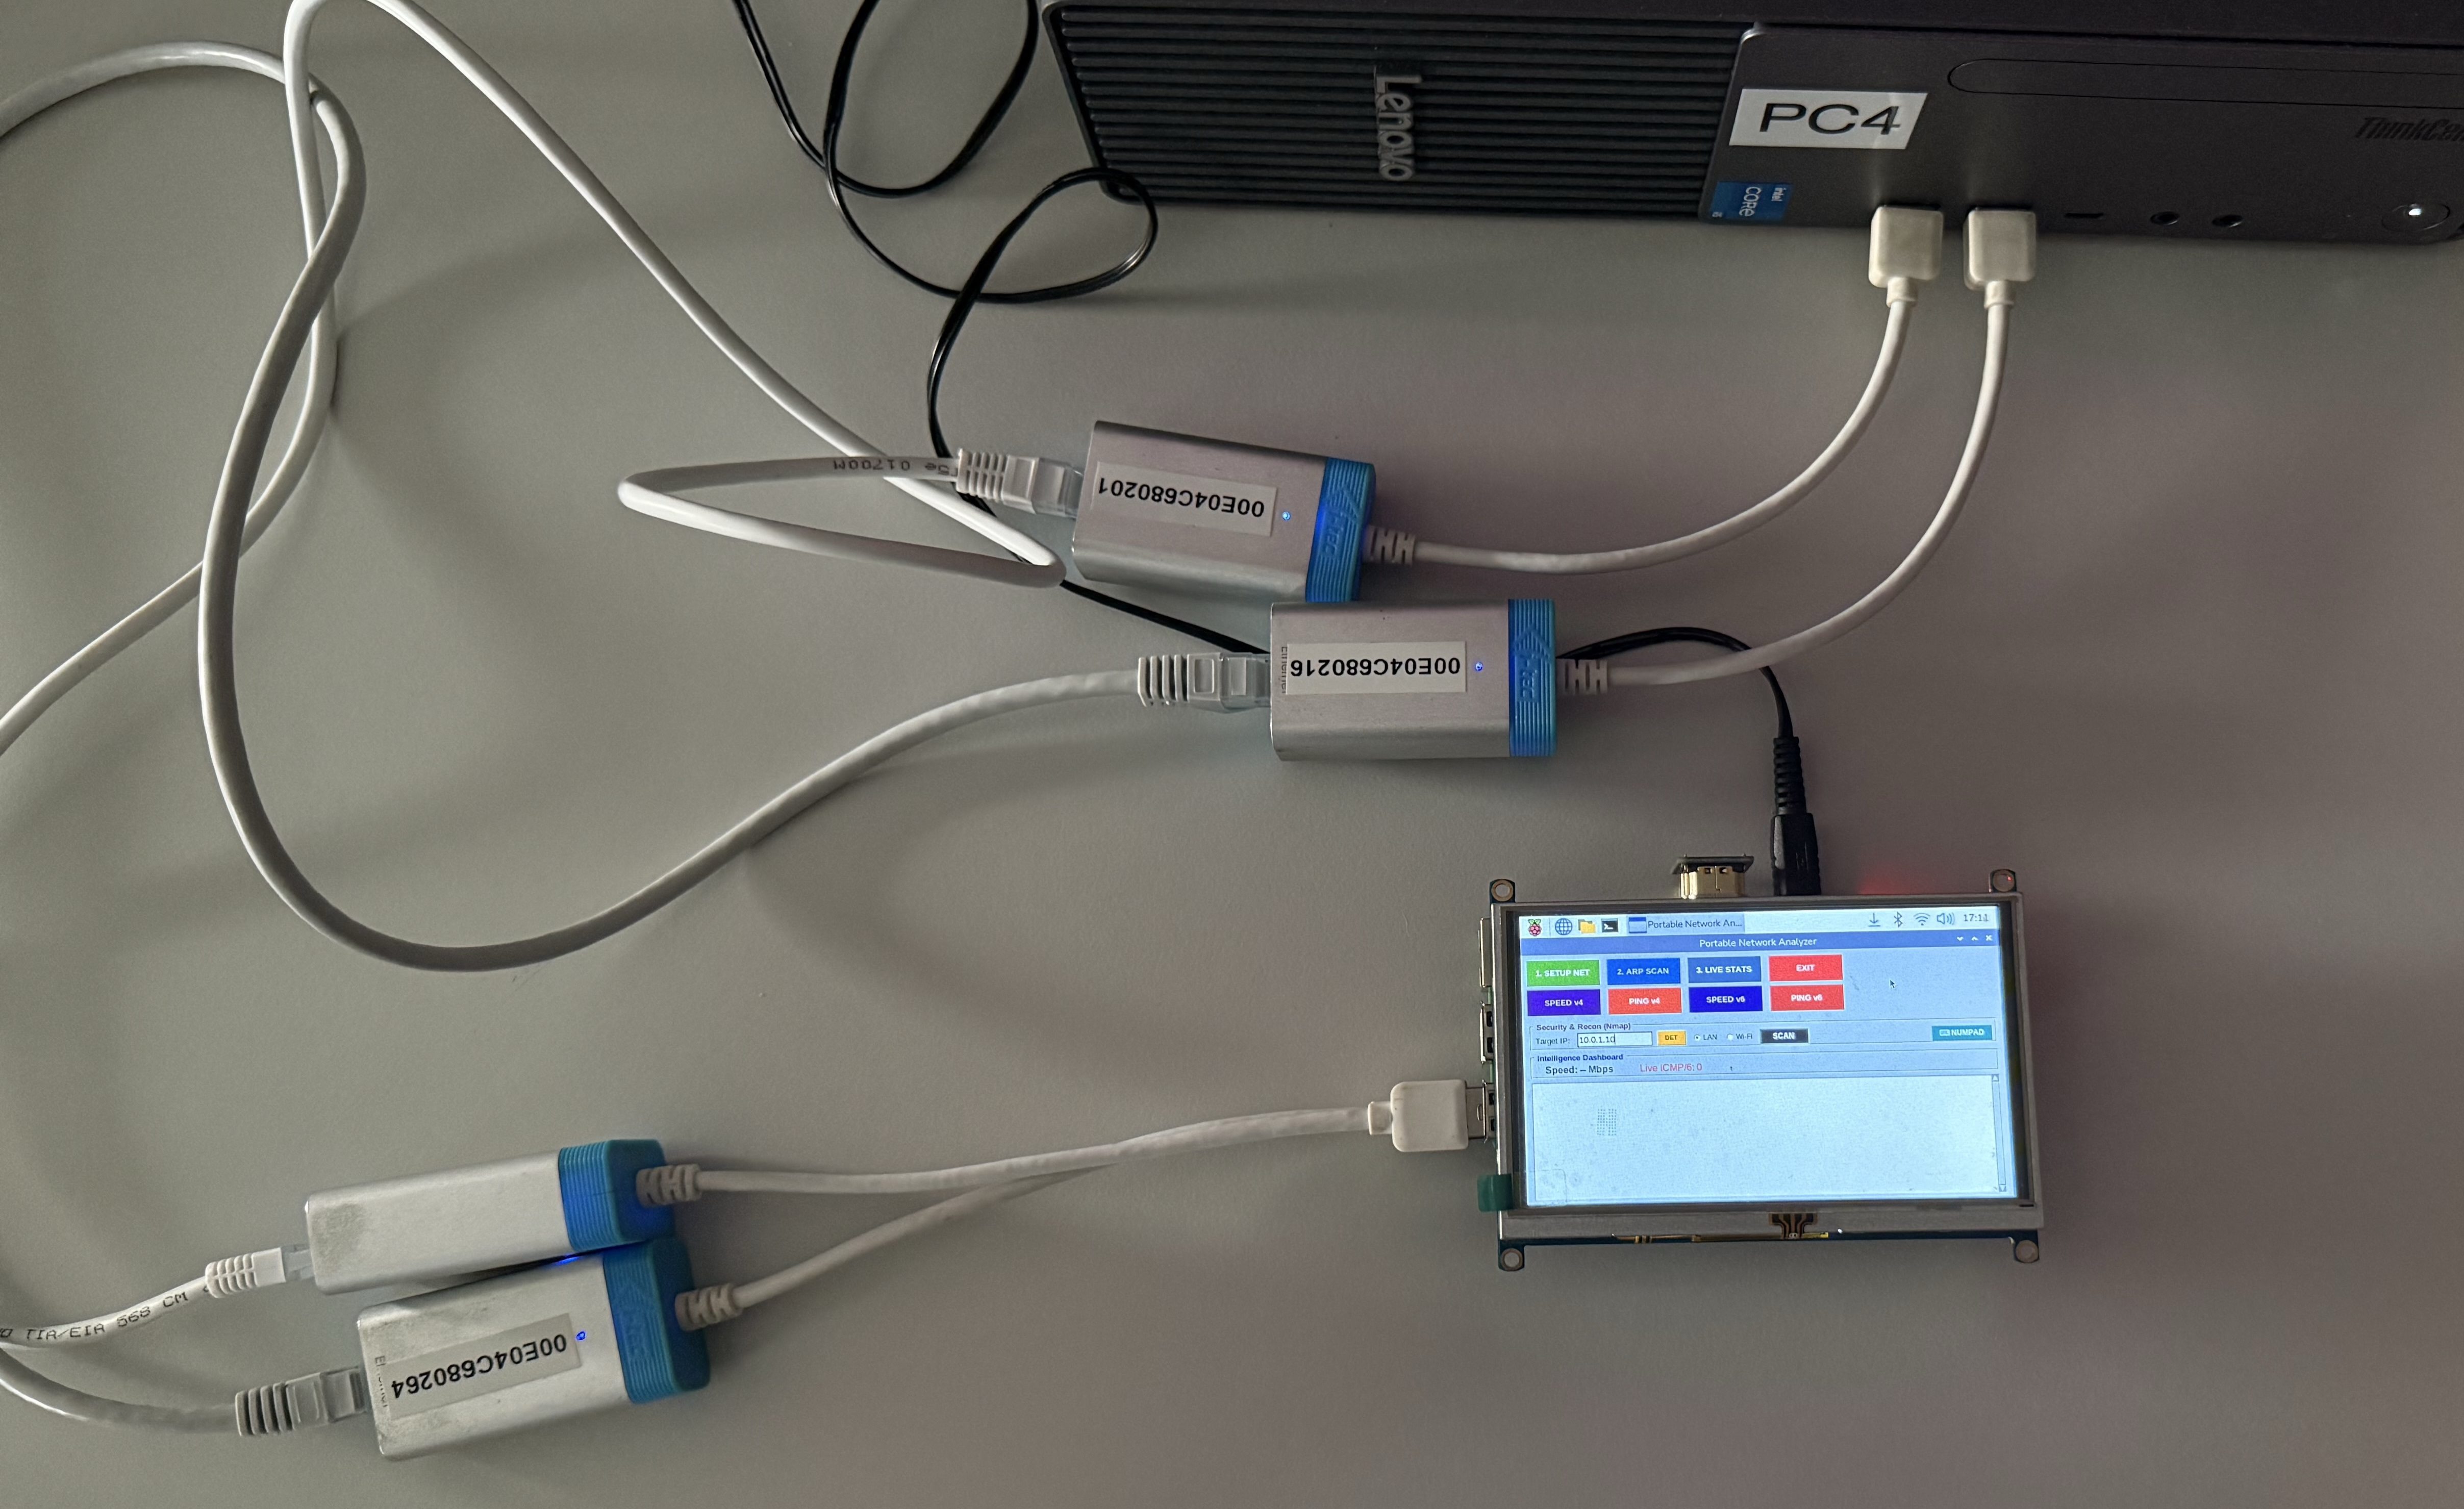
\includegraphics[width=0.85\textwidth, angle=0]{Figures/connected_device.JPG}
    \caption{Fyzické zapojení analyzátoru a cílové stanice v laboratoři}
    \label{fig:zapojeni}
\end{figure}

\subsection{Ověření automatické konfigurace adres}
\label{sec:overeni_autokonfigurace}

Chování adresní autokonfigurace popsané v podkapitole \ref{sec:autokonfigurace} bylo ověřeno samostatným měřením, při němž byl analyzátor propojen s cílovou stanicí oběma testovacími porty současně. Uspořádání měření umožnilo porovnat obě konfigurace na jediném zařízení a ve stejném okamžiku: monitorovací port byl restartován s doplněným klíčovým slovem \texttt{slaac}, zatímco port pro generování provozu byl ponechán v původním nastavení jako kontrolní vzorek. Výsledné adresy přidělené oběma rozhraním cílové stanice shrnuje Tabulka \ref{tab:adresy}.

\begin{table}[htbp]
    \caption{Adresy přidělené cílové stanici na obou testovacích portech}
    \label{tab:adresy}
    \centering
    \begin{tabular}{lll}
        \hline
        Port analyzátoru & Adresa cílové stanice & Způsob získání \\
        \hline
        monitorovací, A = 1 & \texttt{10.0.1.20} & DHCPv4 \\
        monitorovací, A = 1 & \texttt{fd00:1::20/128} & stavově, DHCPv6 \\
        monitorovací, A = 1 & \texttt{fd00:1::2e0:4cff:fe68:216/64} & bezstavově, jádrem ze zprávy RA \\
        generující, A = 0 & \texttt{10.0.2.20} & DHCPv4 \\
        generující, A = 0 & \texttt{fd00:2::20/128} & stavově, DHCPv6 \\
        \hline
    \end{tabular}
\end{table}

Rozdíl mezi oběma řádky s protokolem IPv6 je podstatou celého měření. Na monitorovacím portu vznikla vedle stavově přidělené adresy také adresa sestavená jádrem z inzerovaného prefixu, kdežto na kontrolním portu se zhasnutým příznakem A žádná taková adresa nevznikla, přestože obě rozhraní byla po celou dobu ve stavu \texttt{UP} a obsluhována týmž zařízením. Doplnění jediného klíčového slova do konfigurace serveru dnsmasq je tedy skutečnou a jedinou příčinou pozorované změny.

Následně byly provedeny testy dostupnosti (ICMP Echo Request pro IPv4 a ICMPv6 pro IPv6), a to jak na adresy přidělené stavově, tak na adresu sestavenou bezstavově. Všechna měření potvrdila stabilní spojení s nulovou ztrátovostí paketů a dobou odezvy pohybující se okolo jedné milisekundy (viz Obrázky \ref{fig:pingv4} a \ref{fig:pingv6}).

\begin{figure}[htbp]
    \centering
    \includegraphics[width=0.8\textwidth]{Figures/gui_pingv4.JPG}
    \caption{Test dostupnosti cílové stanice protokolem IPv4}
    \label{fig:pingv4}
\end{figure}

\begin{figure}[htbp]
    \centering
    \includegraphics[width=0.8\textwidth]{Figures/gui_pingv6.JPG}
    \caption{Test dostupnosti cílové stanice protokolem IPv6}
    \label{fig:pingv6}
\end{figure}

Samostatně byla ověřena také funkce mapování topologie realizovaná knihovnou Scapy. Skenování protokolem ARP provedené uvnitř izolovaného jmenného prostoru nalezlo v testovaném segmentu právě jednu stanici a vypsalo její fyzickou adresu (viz Obrázek \ref{fig:arp_scan}), což odpovídá skutečnému zapojení laboratorního stanoviště.

\begin{figure}[htbp]
    \centering
    \includegraphics[width=0.8\textwidth]{Figures/gui_arp_scan.JPG}
    \caption{Výsledek skenování protokolem ARP v izolovaném jmenném prostoru}
    \label{fig:arp_scan}
\end{figure}

\subsection{Ověření auditu protokolu IPv6}
\label{sec:overeni_auditu}

Modul auditu popsaný v podkapitolách \ref{sec:audit_ra} a \ref{sec:vyhledavani_sousedu} byl ověřen v uspořádání, které si vyžádalo výše uvedené omezení, totiž propojením obou testovacích portů jediným kabelem přímo mezi sebou. Obě linky se ustavily na rychlosti 1000 Mbps v plně duplexním režimu. Uspořádání přineslo vedle vlastního ověření také nezávislé potvrzení dřívějšího pozorování: jakmile byl kabel zapojen, sestavilo si jádro analyzátoru na obou rozhraních adresy z prefixů ohlašovaných protějším portem a označilo je příznakem \texttt{proto kernel\_ra}. Protistrana pro následné testy tedy nevznikla ručním nastavením, nýbrž samočinně.

Rozbor zprávy Router Advertisement zachycené na generujícím portu je zachycen na Obrázku \ref{fig:ra_scan}. Přístroj správně určil, že ohlašující směrovač je jeho vlastní monitorovací port, neboť fyzická adresa odesílatele odpovídá jednomu z jeho rozhraní a zpráva byla přijata po vedení, nikoli odeslána tímtéž portem. Z obsahu zprávy byl vyčten inzerovaný prefix \texttt{fd00:1::/64} s dobou platnosti 43\,200 sekund, hodnota MTU 1500 bajtů a doba platnosti směrovače 1800 sekund.

\begin{figure}[htbp]
    \centering
    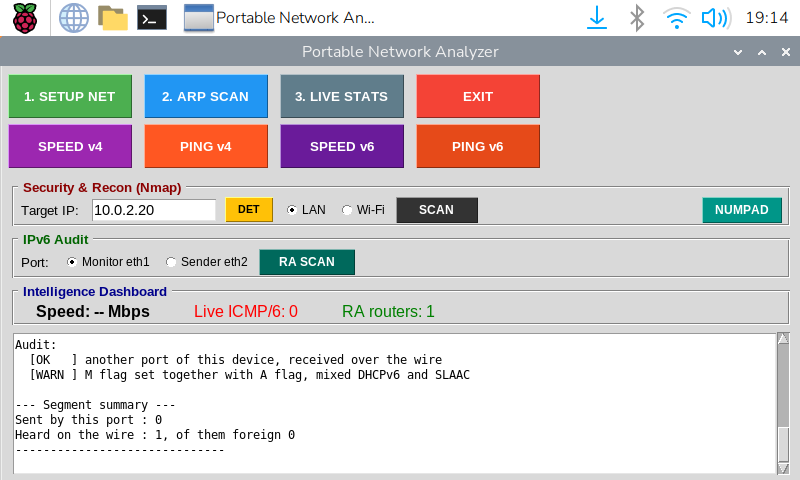
\includegraphics[width=0.8\textwidth]{Figures/gui_ra_scan.png}
    \caption{Rozbor zprávy Router Advertisement zachycené druhým portem analyzátoru}
    \label{fig:ra_scan}
\end{figure}

Teprve toto uspořádání umožnilo ověřit chování popsané v podkapitole \ref{sec:autokonfigurace} měřením provedeným samotným přístrojem, tedy bez pomoci nástrojů nainstalovaných na cílové stanici. Byla-li konfigurace serveru dnsmasq ponechána v původním tvaru, ohlásil audit u inzerovaného prefixu zhasnutý příznak A a vypsal upozornění, že bezstavová autokonfigurace je zakázána. Po doplnění klíčového slova \texttt{slaac} do téhož parametru ohlásil týž prefix s příznakem A zdviženým. Hodnoty uvedené v Tabulce \ref{tab:ra_flags} jsou tak potvrzeny druhým, nezávislým měřením.

Audit zároveň upozornil na okolnost, která při dřívějším měření zůstala nepovšimnuta. Server dnsmasq po doplnění klíčového slova \texttt{slaac} nadále nastavuje příznak M a současně zdvihá příznak A, takže cílové stanici nabízí oba zdroje adresy zároveň, stavový i bezstavový. Nejde o vadu přístroje ani o chybu v rozboru, nýbrž o přesný popis toho, jak se použitý server chová; přijímající stanice pak podle vlastní implementace může získat adresy obě, což je také přesně to, co bylo v Tabulce \ref{tab:adresy} pozorováno.

Samotné kontroly nebylo možné ověřit na skutečném provozu, neboť v testovaném segmentu se žádný nesprávně nastavený ani cizí směrovač nevyskytuje. Byly proto ověřeny na programově sestaveném pracovišti tvořeném dvojicí dočasných jmenných prostorů spojených virtuálním párem rozhraní, do něhož byla vložena záměrně vadná zpráva. Ta nesla hodnotu Cur Hop Limit 64 namísto předepsaných 255, zdrojovou adresu mimo rozsah lokální linky, prefix délky 48 bitů se zdviženým příznakem A, preferovanou dobu životnosti vyšší než dobu platnosti, hodnotu MTU 1200 bajtů a fyzickou adresu ve volbě odlišnou od adresy v rámci. Přístroj označil všechny uvedené nesrovnalosti současně a zprávu vyhodnotil jako pocházející od cizího směrovače.

Funkce vyhledání protistrany byla ověřena na témže vedení. Přístroj nalezl jediného souseda, dopočetl z jeho fyzické adresy identifikátor rozhraní a zjistil, že se shoduje s adresou lokální linky, kterou soused používá; ohlásil tedy klasický postup podle fyzické adresy, nikoli identifikátor podle \cite{rfc7217}. Pro oba prefixy nastavené na portu sestavil odpovídající adresu a obě ověřil jako dosažitelné (viz Obrázek \ref{fig:neigh_scan}). Následný test dostupnosti již proběhl na adresu takto nalezenou, nikoli na adresu zapsanou v aplikaci, a skončil bez ztráty paketů (viz Obrázek \ref{fig:ping_discovered}).

\begin{figure}[htbp]
    \centering
    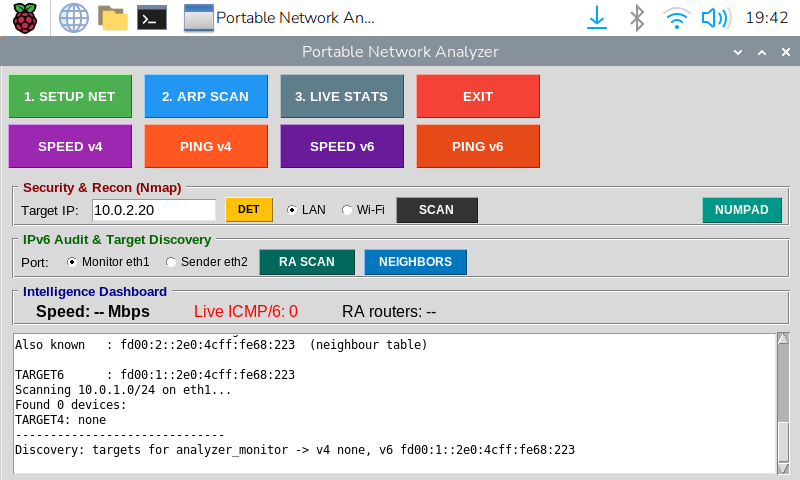
\includegraphics[width=0.8\textwidth]{Figures/gui_neigh_scan.png}
    \caption{Vyhledání sousedů v segmentu a odvození jejich adres postupem EUI-64}
    \label{fig:neigh_scan}
\end{figure}

\begin{figure}[htbp]
    \centering
    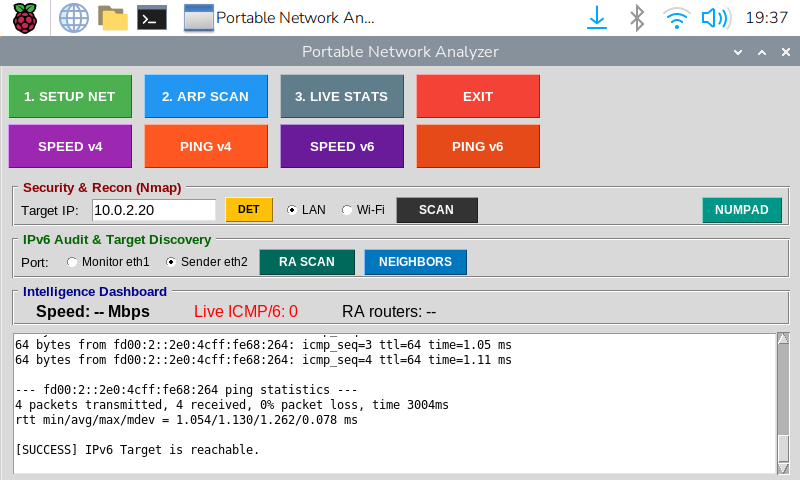
\includegraphics[width=0.8\textwidth]{Figures/gui_ping_discovered.png}
    \caption{Test dostupnosti provedený na adresu nalezenou vyhledáním sousedů}
    \label{fig:ping_discovered}
\end{figure}

Nejcennějším výsledkem tohoto měření je však srovnání obou protokolů provedené na jediném vedení a v jediném okamžiku, které shrnuje Tabulka \ref{tab:sousede}. Skenování protokolem ARP nenalezlo v segmentu žádnou stanici, přestože protistrana byla připojena a odpovídala. Příčina je zřejmá: obě rozhraní náleží odlišným podsítím a na protějším konci neběží žádný klient DHCP, takže adresa z rozsahu monitorovacího portu na něm nikdy nevznikla. Protokol IPv6 nalezl na témže vedení téhož souseda, jeho adresu odvodil z fyzické adresy a ověřil ji testem dostupnosti, a to bez jediného procesu zajišťujícího konfiguraci. Tvrzení vyslovené v podkapitole \ref{sec:autokonfigurace} je tak podloženo měřením, nikoli pouze rozborem konfigurace.

\begin{table}[htbp]
    \caption{Vyhledání protistrany na témže vedení oběma protokoly}
    \label{tab:sousede}
    \centering
    \begin{tabular}{lll}
        \hline
        Protokol & Použitý postup & Výsledek \\
        \hline
        IPv4 & skenování ARP v rozsahu \texttt{10.0.1.0/24} & nenalezena žádná stanice \\
        IPv6 & dotaz na \texttt{ff02::1} a tabulka sousedů & nalezen soused, adresa ověřena \\
        \hline
    \end{tabular}
\end{table}

\subsection{Měření propustnosti}
\label{sec:mereni_propustnosti}

Nejvýznamnější částí testování bylo ověření maximální propustnosti sítě pomocí zátěžového generátoru iperf3.

\begin{figure}[htbp]
    \centering
    \includegraphics[width=0.8\textwidth]{Figures/gui_speedv4.JPG}
    \caption{Měření propustnosti sítě protokolem IPv4}
    \label{fig:speedv4}
\end{figure}

Při testování propustnosti nad protokolem IPv4 dosáhla síť průměrné rychlosti 276 Mbps (viz Obrázek \ref{fig:speedv4}). Následný test využívající protokol IPv6 prokázal propustnost 274 Mbps (viz Obrázek \ref{fig:speedv6}). Drobné snížení propustnosti u protokolu IPv6 o 2 Mbps koresponduje s teoretickými předpoklady rozebranými v podkapitole \ref{sec:ipv4_ipv6}, jelikož základní hlavička protokolu IPv6 o velikosti 40 bajtů je dvakrát větší než hlavička protokolu IPv4, což zvyšuje režii na síťové vrstvě.

Naměřené hodnoty je ovšem nutné vztáhnout k možnostem použité platformy. Obě čísla se pohybují těsně pod hranicí 300 Mbps, kterou výrobce uvádí jako nejvyšší dosažitelnou propustnost ethernetového rozhraní připojeného přes sběrnici USB 2.0 \cite{rpi3bplus}. Měření tedy neurčilo propustnost testované linky, nýbrž narazilo na strop samotného analyzátoru. Tato skutečnost nesnižuje hodnotu srovnání obou protokolů, které proběhlo za zcela shodných podmínek na tomtéž hardwaru, vymezuje však oblast použitelnosti přístroje: k ověření funkčnosti spoje, k porovnání protokolů a k odhalení hrubých závad je zařízení způsobilé, k certifikaci gigabitové linky na její jmenovité rychlosti nikoli. Odstranění tohoto omezení by vyžadovalo přechod na novější generaci jednodeskového počítače s ethernetovým řadičem mimo sběrnici USB.

\begin{figure}[htbp]
    \centering
    \includegraphics[width=0.8\textwidth]{Figures/gui_speedv6.JPG}
    \caption{Měření propustnosti sítě protokolem IPv6}
    \label{fig:speedv6}
\end{figure}

\subsection{Skenování sítě a ověření izolace jmenných prostorů}
\label{sec:skenovani}

Kromě měření propustnosti byla otestována také nově integrovaná funkce bezpečnostního skeneru Nmap. Obrázek \ref{fig:nmap_lan} ilustruje výstup skenování cílové stanice přes izolované ethernetové rozhraní, kde analyzátor správně identifikoval otevřený port služby SSH a detekoval operační systém protistrany.

Právě toto testování odhalilo omezení první verze řídicí aplikace. Skener byl v režimu kabelového skenování spouštěn napevno ve jmenném prostoru \texttt{analyzer\_sender}, takže pokus o sken adresy \texttt{10.0.1.20}, jež náleží podsíti monitorovacího portu, skončil hlášením \texttt{failed to determine route} a žádný cíl nebyl prozkoumán. Táž adresa přitom byla ze jmenného prostoru \texttt{analyzer\_monitor} dostupná bez potíží. Chování tedy nebylo poruchou sítě ani cílové stanice, nýbrž důsledkem toho, že mezi oběma jmennými prostory záměrně neexistuje směrovací cesta.

Z hlediska ověření návrhu je tento výsledek cenný, neboť dokládá, že izolace obou prostředí je skutečná a nikoli pouze deklarovaná: provoz z jednoho prostoru se do druhého nedostane ani tehdy, je-li o to výslovně požádáno. Z hlediska použitelnosti nástroje šlo ovšem o vadu, protože část adresního rozsahu zůstávala z rozhraní nedosažitelná. Aplikace byla proto doplněna o metodu \texttt{netns\_for()}, která podle podsítě zadaného cíle vybere odpovídající jmenný prostor a teprve v něm příslušný nástroj spustí. Stejný mechanismus se nyní uplatňuje i u testů dostupnosti a u zátěžových testů nástrojem iperf3. Po této úpravě proběhne skenování adres z obou podsítí bez chyby, aniž by byla izolace jakkoli narušena.

\begin{figure}[htbp]
    \centering
    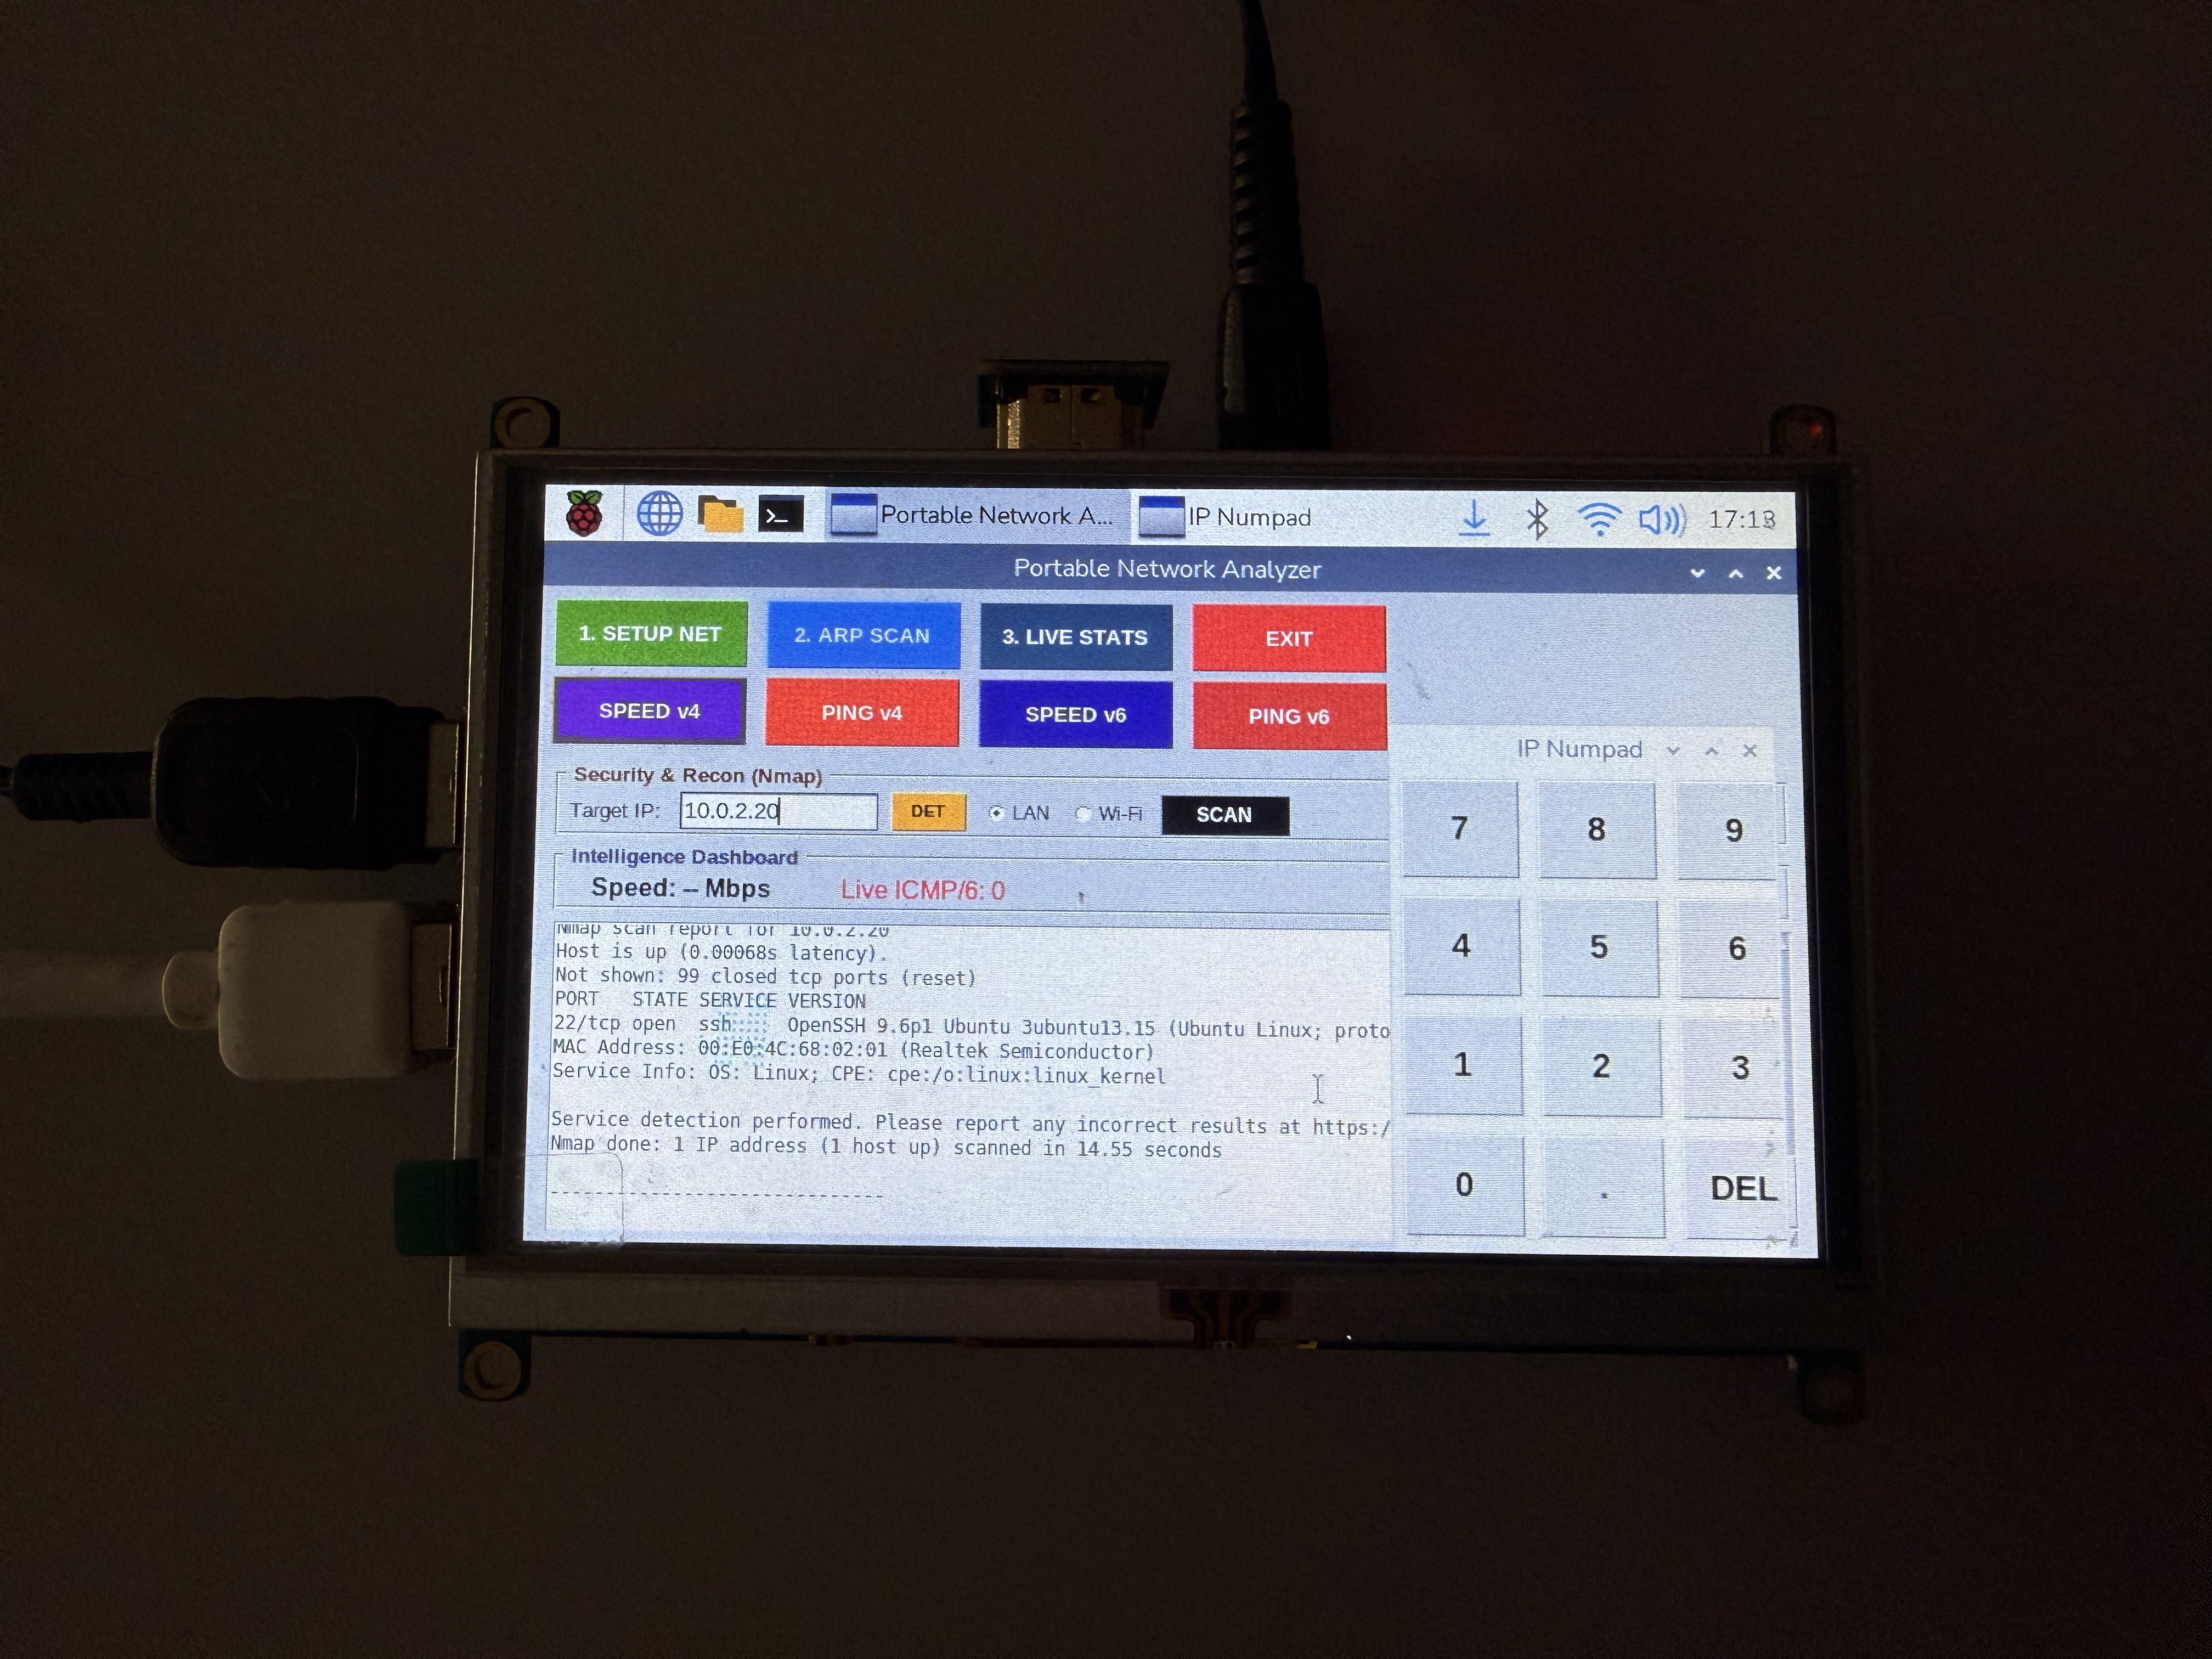
\includegraphics[width=0.8\textwidth]{Figures/gui_nmap_lan_scan.JPG}
    \caption{Výsledek bezpečnostního skenování Nmap v izolovaném prostředí (LAN)}
    \label{fig:nmap_lan}
\end{figure}

Taktéž proběhlo úspěšné ověření bezdrátového průzkumu (viz Obrázek \ref{fig:nmap_wifi}), kde program automaticky detekoval IP adresu přístupového bodu. 

\begin{figure}[htbp]
    \centering
    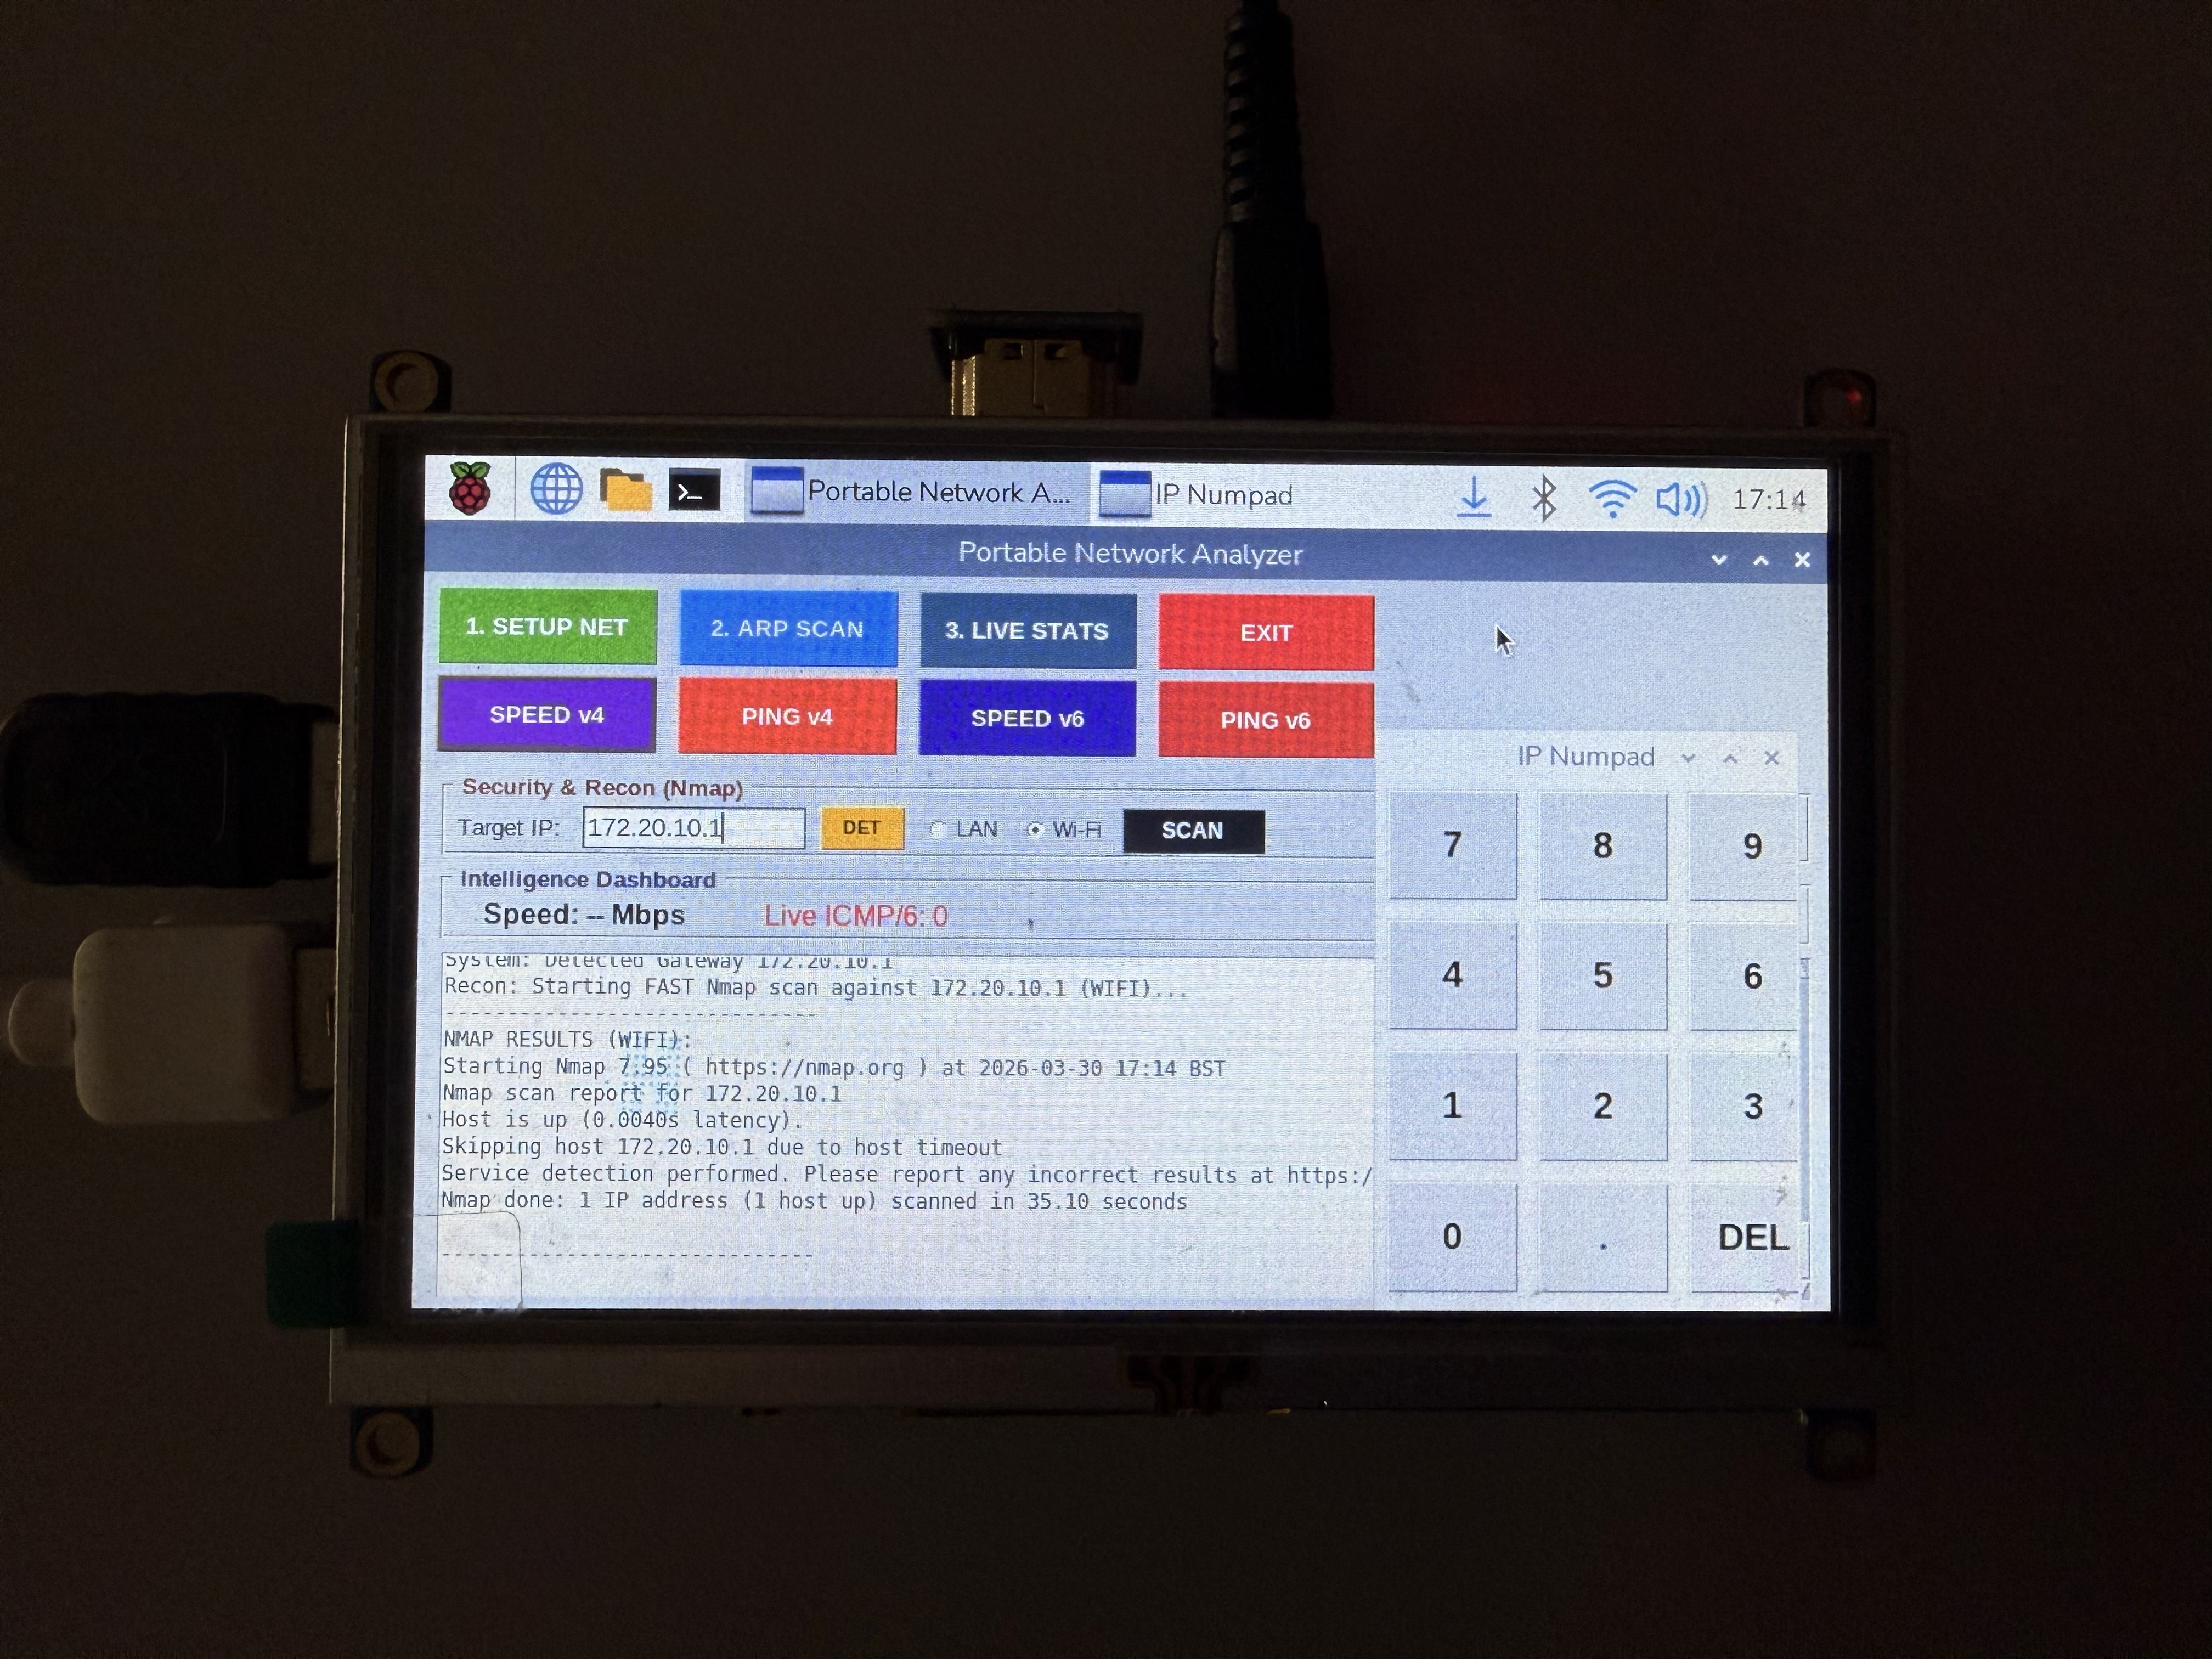
\includegraphics[width=0.8\textwidth]{Figures/gui_nmap_wifi_scan.JPG}
    \caption{Bezdrátové skenování sítě s využitím automatické detekce výchozí brány (Wi-Fi)}
    \label{fig:nmap_wifi}
\end{figure}

Správnost obou zátěžových testů potvrdily také logy zachycené na straně cílového serveru (viz Obrázek \ref{fig:iperf_server}), které prokazují paralelní schopnost analyzátoru pracovat v obou adresních prostorech bez konfliktů ve směrování. Zařízení tak plně splnilo definované cíle.

\begin{figure}[htbp]
    \centering
    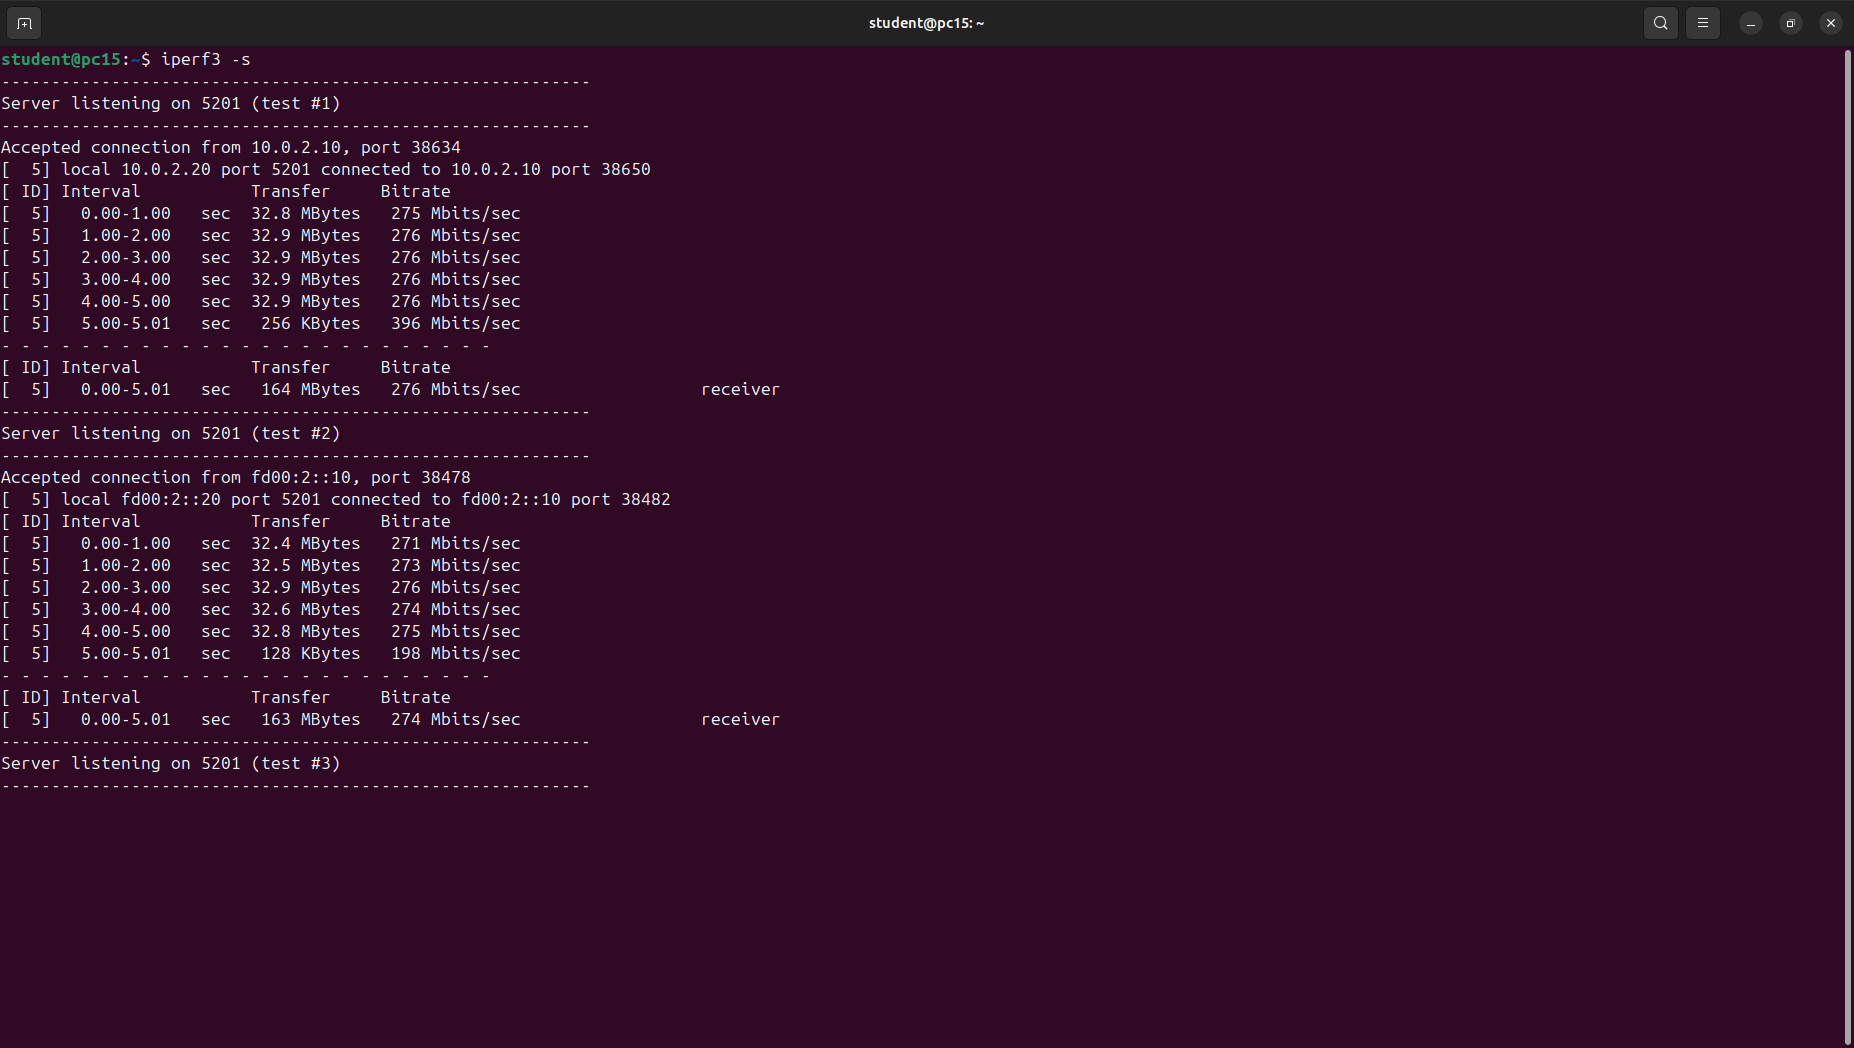
\includegraphics[width=0.9\textwidth]{Figures/iperf_tests.png}
    \caption{Výstup nástroje iperf3 na straně cílového serveru (IPv4 i IPv6 spojení)}
    \label{fig:iperf_server}
\end{figure}

\subsection{Vady odhalené při opakovaném ověřování}
\label{sec:odhalene_vady}

Vedle vady ve výběru jmenného prostoru popsané v podkapitole \ref{sec:skenovani} odhalilo opakované ověřování prototypu ještě dvě další. Obě stojí za uvedení, neboť ani jedna se neprojevila při prvním průchodu měřením a obě mohly zůstat skryté až do nasazení přístroje mimo laboratoř.

První z nich se týkala inicializačního skriptu. Spuštění přípravy síťového prostředí podruhé v témže běhu systému selhalo hlášením, že rozhraní generujícího portu neexistuje, a příslušný jmenný prostor zůstal prázdný. Příčinou je způsob, jakým jádro nakládá s fyzickými rozhraními při rušení jmenného prostoru: rozhraní se do výchozího prostoru vracejí až po dokončení úklidu, tedy s jistým zpožděním, kdežto skript se je pokoušel přesunout okamžitě. První z obou rozhraní se do doby pokusu vrátit stihlo, druhé nikoli. Při prvním spuštění po zapnutí přístroje se vada neprojevila, neboť obě rozhraní se ve výchozím prostoru již nacházela, a proto zůstala až dosud nepovšimnuta. Skript nyní na návrat rozhraní vyčká; opakované spuštění proběhne bez chyby.

Druhá vada se týkala řídicí aplikace a byla odhalena způsobem, který stojí za zaznamenání z metodického hlediska. Na pořízeném snímku obrazovky se výpis jevil jako přerušovaný a část textu se na displeji zdvojovala. Obsah výpisu odečtený programově byl přitom bezvadný, z čehož plyne, že se nejednalo o chybu v datech, nýbrž o chybu vykreslování. Skutečná příčina spočívala v tom, že jednotlivé úlohy zapisovaly do prvků grafického rozhraní přímo z vlastních vláken, což použitá knihovna nepřipouští a co v krajním případě nevede k poškozenému obrazu, nýbrž k pádu aplikace. Zápis do prvků rozhraní je proto nyní odkládán do hlavního vlákna. Poznatek je obecnější než tento konkrétní případ: jeví-li se výstup na displeji podezřele, je namístě porovnat jej s daty a nespoléhat na to, co je vidět.